\chapter{Conclusion}

So what does the data show us regarding the current capabilities of our all-sky camera setup? There are improvements to be made, problems to troubleshoot, but on a wholistic sense, the system and software seems most assuredly capable of photometrically analyzing the events.

\section{Critique}
One potentially problematic issue is there is currently no way for us to compare our calibrated light curves to other calibrated magnitudes. Each of the potential ways to do so are somewhat flawed in one aspect or the other. Comparing our data to NASA's allows us to effectively see if the shape of our light curve is accurate, but as their posted data is uncalibrated to a reference object, we cannot confirm our calibration. The other source of comparison is the Iridium flare data. The Iridium flare data does not have light curves to compare to but they do have posted maximum magnitudes. Unfortunately, as mentioned in the data section, our camera cannot see that maximum magnitude in most Iridium flare events due to oversaturation. For future events, it would be worthwhile to attempt at adjusting the sensitivity levels of the camera. The only other option would be extrapolating the peaks from the Gaussian curves, but that creates more accuracy issues as previously mentioned.

In order to confirm our calibration is accurate, we should find data sets with calibrated magnitudes and posted video clips to compare to. However, it is worth noting that if the program can detect the shape of the light curve accurately, which it has repeatedly shown it can, it should have no problem with the calibration. After all, the calibration is dependent on the same algorithm, only it arises from the calculation of the reference star's magnitude instead of the object's magnitude. In fact, it should be even easier to do so, as the reference star does not move throughout the duration of the event; the program does not need to update the position it is covering. 

There is also potentially more data to gain from the reference objects as well. As mentioned in the Chapter 4, there are often multiple reference objects seen in the video. Calibrating off of multiple reference objects would give us greater confidence in the calibration capabilities. As those objects' magnitudes should be constant throughout the event, their light curves could also allude to the margin of error in our light curves depending on how nonlinear their light curves appear.

\subsection{Atmospheric Extinction}
Further examination is needed to figure out whether or not the discrepancies at the beginning of the light curve is based off a correctable parameter such as atmospheric extinction, or whether it arises from a systematic failure in the program to successfully find the magnitudes of dimmer objects.

We most likely will have to account for atmospheric extinction. Atmospheric extinction, visualized in \ref{fig:extinction}, is a phenomenon caused by different areas of the sky having different amounts of air between them and the observer. As a result, a meteor near the horizon is separated by more air, and thus appears dimmer than if the same meteor was right above the observer. 
\begin{figure}[ht!]
	\centering
	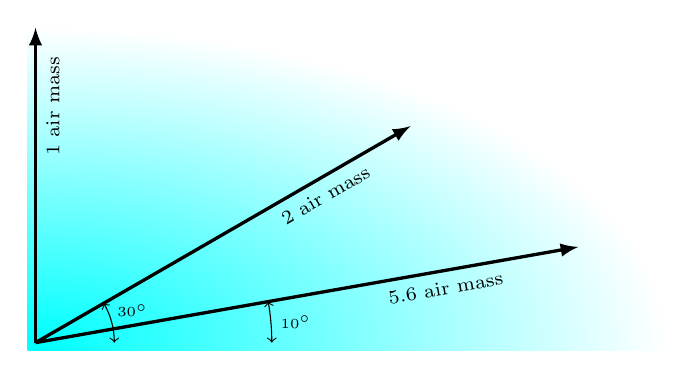
\begin{tikzpicture}
		\clip (-.1,-.1) rectangle (8,4);
		\shade[inner color=cyan, outer color=white] (0,0) ellipse (8cm and 4cm);
		\draw[-latex, very thick] (0,0) -- (90:4) node[near end, font=\scriptsize, sloped, below]{1 air mass};
		\draw[-latex, very thick] (0,0) -- (30:5.5cm) node[near end, font=\scriptsize, sloped, below]{2 air mass};
		\draw[-latex, very thick] (0,0) -- (10:7cm) node[near end, font=\scriptsize, sloped, below]{5.6 air mass};
		\draw[<->] (0,0) ++(1,0) arc (0:30:1) node[pos=.8, right, font=\tiny]{$30^{\circ}$};
		\draw[<->] (0,0) ++(3,0) arc (0:10:3) node[midway, right, font=\tiny]{$10^{\circ}$};
	\end{tikzpicture}	
	\caption{There is more air in between someone and an object along the horizon than an object directly above them.}
	\label{fig:extinction}
\end{figure}


\section{Outlook}
This project is far from being completed. Creating a program that successfully analyzes meteor events is the most important building block for collecting data, but there is much more to do beyond that. Now that the script is set up, a substantial number of events would need to be collected with our own all-sky camera to be able to make any reasonable conclusions about the near-Earth population. If we are able to do so, we are then able to show that a setup similar to D6 is a viable alternative to the larger setups currently in place.  The data that is needed to be collected is the photometric data of the events, but there is substantial statistical analysis that needs to be done to extrapolate that photometric data into meteor size. The future of this project is thus based on optimizing the data collected and analyzing that data to justify drawing any reasonable conclusion.
